\chapter{Methodology}

\section{Intent}

To provide a practical component to this report, we intend to design and implement a generic technological solution that connects an NFP directly to those experiencing homelessness. We believe that this practical implementation will enable us to extend our investigation to include the entire life cycle of a technology based solution in this space. In designing and developing the application we will be exposed to the processes and considerations which lead to a realised product; this exposure will be from both the NFP, and from those experiencing homelessness. Further to these initial phases of the product, we will also be involved in the delivery and roll-out strategies for this application; and will study the implications and receptions to these strategies from both perspectives. Lastly, we will discuss the process of iterating on the application, through the facilitation of an ongoing feedback loop between the NFP, the users, and the developers.

Using this approach, we aim to further some understandings already presented in the literature. We believe that this method of undertaking will also give us the most exposure to all facets of the technology life cycle in this space and will therefore provide us with the greatest potential for unexpected or unforeseen learnings. Additionally, to this process providing eventual academic findings, we also aim to provide mutual benefit to both the NFP and the individuals experiencing homelessness who participate in our program. We do not believe it to be ethically viable to perform this study without a primary focus of providing actual recognised benefit to all participants. In discussion of our results, we will also critique our success in providing this benefit.

\section{Requirements}

In an effort to simplify the design process, it was apparent that a core problem area and the surrounding development context must be identified as early as possible. Working with Brisbane based NFP Orange Sky, as well as acknowledging the technical and logistical limitations of their services, particularly as they relate to COVID-19 response efforts, we were able to immediately narrow our scope. The remainder of this section outlines the initial statement of scope, and subsequently discusses its further distillation into a concrete design.

\subsection{Problem Area}

It was well established by Orange Sky, an NFP with a proud mission of \emph{Positively Connecting Communities}, that an emphasis on interpersonal connection would be seen as immensely beneficial to the organisation. It was also established that Orange Sky stakeholders could be separated into the following five groups:

\begin{itemize}
    \item \emph{Friends}: A term used to describe any users of the Orange Sky services, as well those who visit shift but do not participate directly. Usually synonymous with those experiencing homelessness, but also extending to the financially insecure, nomads, and others in need of service.
    \item \emph{Volunteers}: The heart and soul of Orange Sky, with the day-to-day services entirely run by over 2000 volunteers across Australia and New Zealand. Each shift is usually accompanied by anywhere from two to ten or more volunteers,
    \item \emph{Donors}: Those responsible for keeping Orange Sky running every day, usually through financial backing but also occasionally through other tangible support.
    \item \emph{Staff}: The team employed by Orange Sky to do everything from building the vans to operating payroll. Primarily based in a head office in Albion, Brisbane, but also distributed throughout Australia and New Zealand.
    \item \emph{Followers}: Generally speaking, this group encompasses any stakeholder within Orange Sky who does not fit into the above groups. Although these individuals may not use, operate, fund, or work for Orange Sky, they may be a devout supporter on social media or something similar.
\end{itemize}

If we were to consider all possible connections of two stakeholders within the Orange Sky community, including self-referential connection within a single group, there are 15 possible types of connections involving just two stakeholders. Working with the knowledge of the operational model of Orange Sky, we aim to identify some gaps that may exist in these 15 combinations, and will ultimately aim to bridge these gaps through the implementation of connecting technology. We note that as with the rest of this study, we have an explicit affinity towards connecting those experiencing homelessness, and will thus consider the connections not involving this group to be outside the scope of this design. However, to have a comprehensive understanding of Orange Sky, we have still documented these out of scope connections in Table \ref{connectiontable}.

\begin{table}[h]
    \rowcolors{2}{lightgray!50!white!50!}{white}
    \centering
    \begin{tabularx}{\textwidth}{ c | c | Y | c | c }
        \hline
        A          & B          & Connection                                                                                       & Tech & Flow                    \\ [0.5ex]
        \hline
        Friends    & Friends    & In person connection on shift                                                                    & No   & A$\longleftrightarrow$B \\
        Friends    & Volunteers & In person connection on shift                                                                    & No   & A$\longleftrightarrow$B \\
        Friends    & Donors     & Friend stories distributed to donors                                                             & Yes  & A$\longrightarrow$B     \\
        Friends    & Staff      & ---                                                                                              & ---  & ---                     \\
        Friends    & Followers  & Friend stories shared publicly                                                                   & Yes  & A$\longrightarrow$B     \\
        Volunteers & Volunteers & In person connection on shift                                                                    & No   & A$\longleftrightarrow$B \\
        Volunteers & Donors     & Volunteer stories distributed to donors                                                          & Yes  & A$\longrightarrow$B     \\
        Volunteers & Staff      & ---                                                                                              & ---  & ---                     \\
        Volunteers & Followers  & Volunteer stories shared publicly                                                                & Yes  & A$\longrightarrow$B     \\
        Donors     & Donors     & ---                                                                                              & ---  & ---                     \\
        Donors     & Staff      & Donation messages distributed to staff as well as staff directly contacting donors to say thanks & Yes  & A$\longleftrightarrow$B \\
        Donors     & Followers  & Large or interesting donation stories shared publicly                                            & Yes  & A$\longrightarrow$B     \\
        Staff      & Staff      & In person connection in the workplace                                                            & No   & A$\longleftrightarrow$B \\
        Staff      & Followers  & Staff stories shared publicly                                                                    & Yes  & A$\longrightarrow$B     \\
        Followers  & Followers  & ---                                                                                              & ---  & ---                     \\
        \hline
    \end{tabularx}
    \caption{Connections between stakeholder groups facilitated by Orange Sky}
    \label{connectiontable}
\end{table}

It is important to emphasise that Table \ref{connectiontable} simply documents the connections that are directly facilitated by Orange Sky as part of their operating model. This is not to say that other connections do not occur, such as followers interacting with each other on social media, however these extra connection mechanisms are not occurring as a direct result of Orange Sky's model.

Of most interest to our project, based on the prior findings and discussion in this report, are rows in which some or all of following criteria is met:

\begin{enumerate}
    \item There are no existing directly supported connection mechanisms.
    \item The supported connection mechanisms are unidirectional in nature.
    \item The supported connection mechanisms are not underpinned by technology.
    \item \emph{Friends} are at least one of the stakeholder groups (must be met).
\end{enumerate}

Whilst the mutual exclusivity present in these criteria results in no one row being able to meet all points, the connection combinations which we can extract as being most relevant to our work are:

\begin{itemize}
    \item \emph{Friends} \& \emph{Friends}: No technological implementation
    \item \emph{Friends} \& \emph{Volunteers}: No technological implementation
    \item \emph{Friends} \& \emph{Donors}: Unidirectional flow
    \item \emph{Friends} \& \emph{Staff}: No direct mechanisms
    \item \emph{Friends} \& \emph{Followers}: Unidirectional flow
\end{itemize}

It is immediately evident that every single combination involving the \emph{Friends} stakeholder group has been identified as meeting the criteria necessary for being included in the further design of this project. Whilst this connection analysis was not capable of narrowing down our scope, we now have a greater understanding of the wider landscape of Orange Sky, and also have a more detailed understanding of the connection shortcomings for \emph{Friends}.

To tighten the scope of our project before continuation, it was collectively decided that the criteria of unidirectional flow would be dropped, based on the reasoning that rows meeting solely these criteria were at least providing some form of technology based connection. Upon tightening these criteria, we were able to more concisely define our problem area in the following statements:

\begin{itemize}
    \item The primary focus of our application is on connection throughout the Orange Sky community as experienced by \emph{Friends}.
    \item The Orange Sky community will be considered to exist of \emph{Friends}, \emph{Volunteers}, and \emph{Staff} for the purpose of this application. \emph{Donors} and \emph{Followers} will not be considered directly.
\end{itemize}

These statements will be the main reference point for the following design discussion, in which specific requirements will be distilled. The statements that did meet some criteria, but where subsequently filtered out for this project, provide an excellent platform for future work.

\subsection{Non-functional Requirements}

Based on the operational models and geographical distribution of Orange Sky's services, it was necessary to identify some fundamental non-functional requirements that will shape the overall composition of our application. These requirements are outlined in Table \ref{nonfunctionalreqs}.

\begin{table}[h]
    \rowcolors{2}{lightgray!50!white!50!}{white}
    \centering
    \begin{tabularx}{\textwidth}{ >{\hsize=0.3\hsize}Y | >{\hsize=0.7\hsize}Y }
        \hline
        Requirement                                                       & Reasoning                                                                                                                                                                                                                                                                                                                                 \\ [0.5ex]
        \hline
        Application must run on 7” Android Tablet running Android Oreo Go & Orange Sky use this type of tablet readily in their services; as such, delivery and participation will be streamlined by accommodating for this device specification                                                                                                                                                                      \\
        All data must be stored remotely and securely                     & Orange Sky do not provide physical theft protection mechanisms on their existing devices. Orange Sky's model revolves around all important data being immediately offloaded to the cloud, such that theft of a tablet would not be a loss or unintended disclosure of any data. We will aim to replicate this security and privacy model. \\
        Internet connection required at all times                         & To accommodate for the previous requirement, it will be necessary for our application to be deployed in an environment with a constant internet connection.                                                                                                                                                                               \\
        No identifying information may be intentionally collected         & Protecting the right to anonymity that all Orange Sky \emph{Friends} have is extremely important to the organisation. Whilst we cannot prevent anyone from sharing this information if free text or audio input is allowed in our application, we will not encourage or require the collection of any such information.                   \\
        \hline
    \end{tabularx}
    \caption{Non-functional requirements of our application.}
    \label{nonfunctionalreqs}
\end{table}

\subsection{User Stories}

Enhanced understanding of the problem area, and simultaneously the next phase of design, involved empathising with the potential users of this application through the distillation of user stories.
These user stories were developed through consultation with experts within the Orange Sky environment, as well as through the knowledge that was established during our review of existing literature.
These user stories follow the generally accepted pattern of \emph{“As \dots, I want \dots so that \dots”} and are listed below.

\begin{itemize}
    \item \emph{As} a local friend, \emph{I want} to share my stories with others in my local community \emph{so that} shared experiences can be established in my local community of friends.
    \item \emph{As} local friend, \emph{I want} read and empathise with other stories from my local community \emph{so that} I can better understand my local community's experiences.
    \item \emph{As} an Orange Sky friend, \emph{I want} share my experiences with Orange Sky HQ \emph{so that} they can be heard and understood by those who make shifts happen.
    \item \emph{As} an Orange Sky friend, \emph{I want} share my ideas and opinions with Orange Sky HQ \emph{so that} they can be considered in future decision-making.
    \item \emph{As} a socially disconnected friend, \emph{I want} read stories from all across the country \emph{so that} I can feel connected to those who may be distant, but are still having similar experiences to me.
    \item \emph{As} a socially isolated friend, \emph{I want} share my stories with other friends \emph{so that} I can feel heard.
    \item \emph{As} a storytelling friend, \emph{I want} see who reads my stories, and where they are from \emph{so that} I can feel empowered about my ability to share my stories.
    \item \emph{As} Orange Sky HQ, \emph{I want} read stories shared by friends \emph{so that} I can empathise with their experiences and better deliver our service.
    \item \emph{As} Orange Sky HQ, \emph{I want} to obtain potential storytelling leads \emph{so that} these leads can be further investigated and shared as an Orange Sky case study or story.
    \item \emph{As} a knowledgeable friend, \emph{I want} share important information I have obtained through my experiences \emph{so that} others may also benefit from this knowledge.
\end{itemize}

\section{Proposed Solution: Story Sharing}

Upon analysis of the requirements outlined above, both non-functional and functional, it was concluded that a story sharing application would enable these requirements to be met in their entirety. We also postulate that a story sharing application would also be generic enough in nature to encourage participation from a larger audience, and would also be open to a large amount of iteration and progression over time, encouraging co-design processes and collaborative feedback loops to be established by Orange Sky. Storytelling is at the core of Orange Sky's communication strategies, and thus we also confirm that this proposed application aligns well with wider organisational imperatives. The following sections outline the process of refinement from our abstract requirements to a concrete design right through to our final prototypes to be taken into the field.

\subsection{Use Cases}

Here we list the concrete use cases which our application will implement. These use cases have been extracted from the user stories above, and provide a blueprint for application design and development.

\begin{itemize}
    \item Friends can share stories using the application
    \item Stories will remain anonymous, and should be identified by the Orange Sky shift name, the date and time, and optionally a first name
    \item Shared stories will be viewable in the application
    \item Shared stories must be manually reviewed and approved by a moderation team before they can be viewed in the application
    \item The application will provide important information around maintaining privacy and anonymity when sharing stories, as well as the types of stories which may or may not be appropriate for sharing
    \item The application should make it easy for an administrator to remove or edit stories after they have been shared
    \item Upon viewing a story, the application will track and increment the read count of the story
    \item The ability to give stories Orange hearts will also be implemented as a means of acknowledging the positive reception of a shared story
    \item It will also be visible when viewing a story to see when/where/who initially shared it, as well as when/where/who viewed it, and finally how many Orange hearts it has received
    \item The ability to provide general feedback on the tool will also be present at all times
    \item General information on the tool will be available at all times, such as privacy information, contact information and general help
\end{itemize}

In bringing these use cases into a tangible application, we aimed to first iterate with high fidelity mockups. These mockups provided enough context that they were able to be used for obtaining feedback from potential users. This feedback would then be used to update the designs, and this process would continue until such a point where the application felt ready to begin functional prototyping. Below we summarise our experiences with this process.

\subsection{Initial Iteration}

Our initial mockups were first conceived using a whiteboard, before being translated into a digital format using online mockup tool \url{moqups.com}. The initial designs are included in Figure \ref{initialdesigns} and focus heavily on the core components within the application, \emph{Login}, \emph{Drawer Content}, \emph{Read}, and \emph{Share}. The branding and stylistic choices made throughout are done so in an attempt to assimilate the application with existing Orange Sky technologies.

\clearpage

\begin{figure}[ht!]
    \centering
    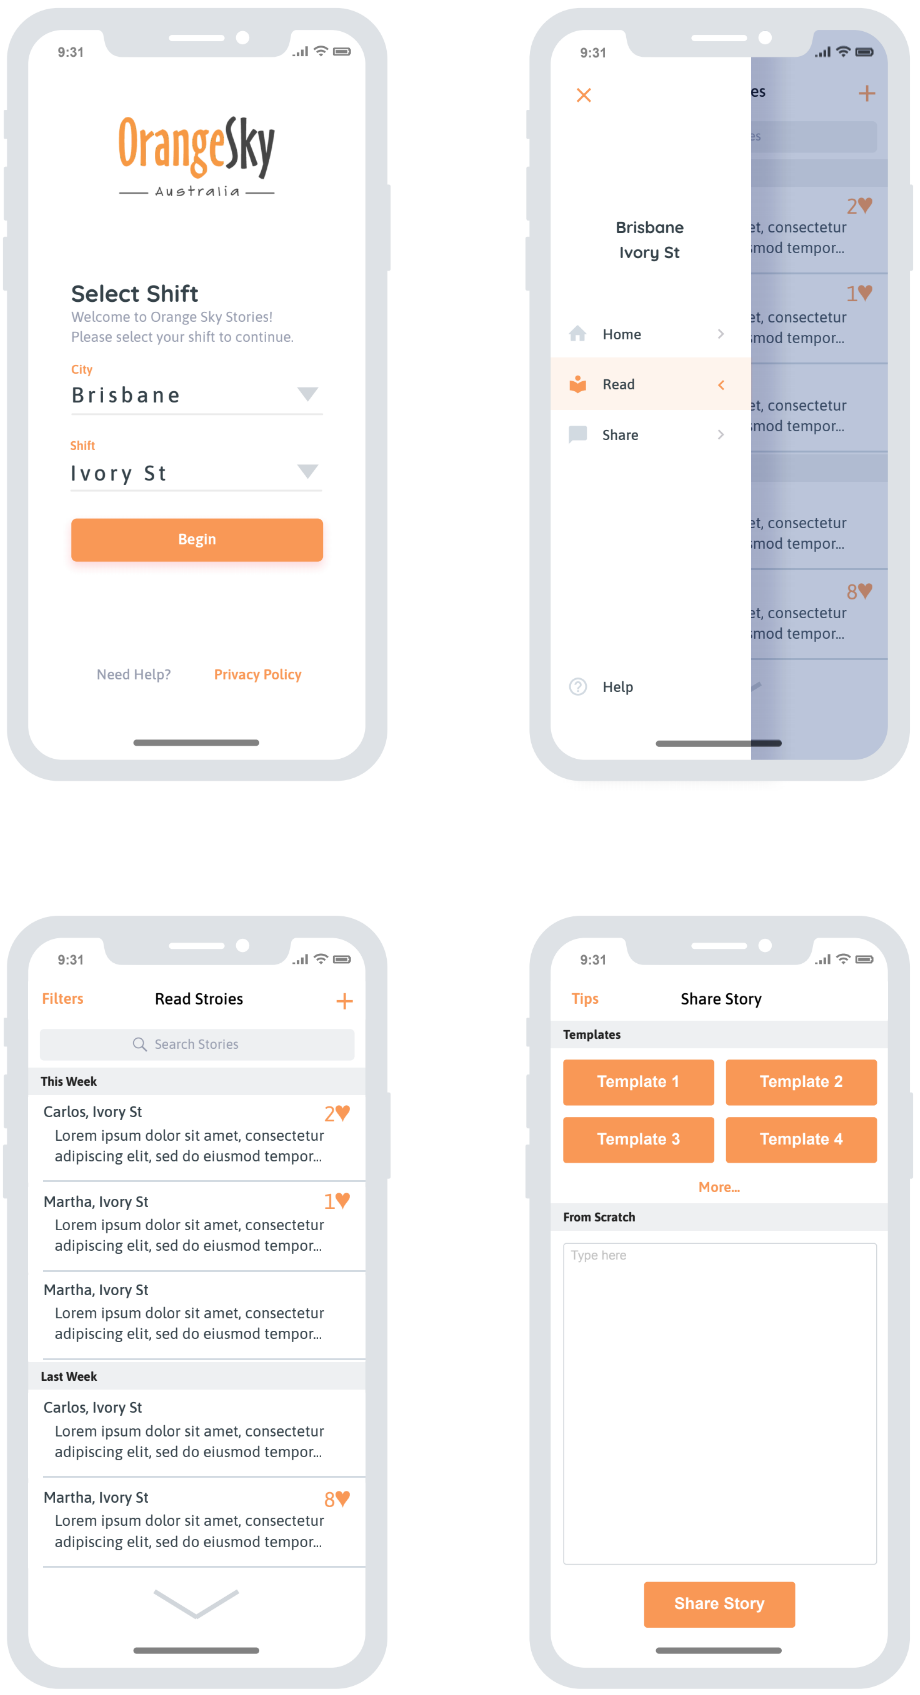
\includegraphics[scale=0.3]{assets/designs/20200816-mockups.png}
    \caption{\centering{Initial Designs: Login (top left), Drawer Content (top right), Read (bottom left), and share (bottom right)}}
    \label{initialdesigns}
\end{figure}

The \emph{Login} screen allows for a number of our use cases to be implemented, including the ability to obtain information about the current use context, as well as the avenue towards providing the current user with important privacy and support information.

The \emph{Drawer Content} provides a navigational element to the application, and also provides the user with an understanding of the core functionality of this application. Support for the user is again readily available on this component. We also note that utilising a navigational drawer, rather than a bottom or top bar, allows for a greater amount of extension in the future. The drawer is capable of accommodating an arbitrary number of additional screens due to its handling of y-dimensional overflow, compared to the limited screen real estate and potential for growth provided by a top or bottom bar.

Our \emph{Read} screen design proposes the utilisation of a reverse chronologically ordered, endlessly scrolling, list of stories. This is a design approach with modern users are extremely comfortable with thanks to the ubiquity of news and social media, and has proven to be successful in these areas. We have also attempted to provide important information on this screen, such that users are able to accurately identify the stories which might appeal most to them. This information consists of data points such as whom, where, and when the story was shared, as well as small preview of the stories content and a small indication of the number of stars that the story has received from readers. This endlessly scrolling list is headed by filter and search options for enhanced user discovery, as well as an \emph{Add} button in the top right to promote the other half of the application's functionality.

Finally, the design for our \emph{Share} screen aims to prompt and encourage an individual aiming to share their story. By providing tips and templates to the user, we believe that this may assist in their synthesis and sharing of their own stories. These templates would be work-shopped and designed alongside experts from Orange Sky, and potential users.

\subsection{Final Prototype}

After a number of iterations aimed at improving our initial designs, based primarily on the feedback of Orange Sky experts, potential users, and the expertise of our supervisor Dr Vyas, a final prototype was established. This prototype represents the design that was ultimately built and distributed as a functional application. Screenshots of this final design are shown in Figure \ref{finalprototype}.

\begin{figure}[ht!]
    \centering
    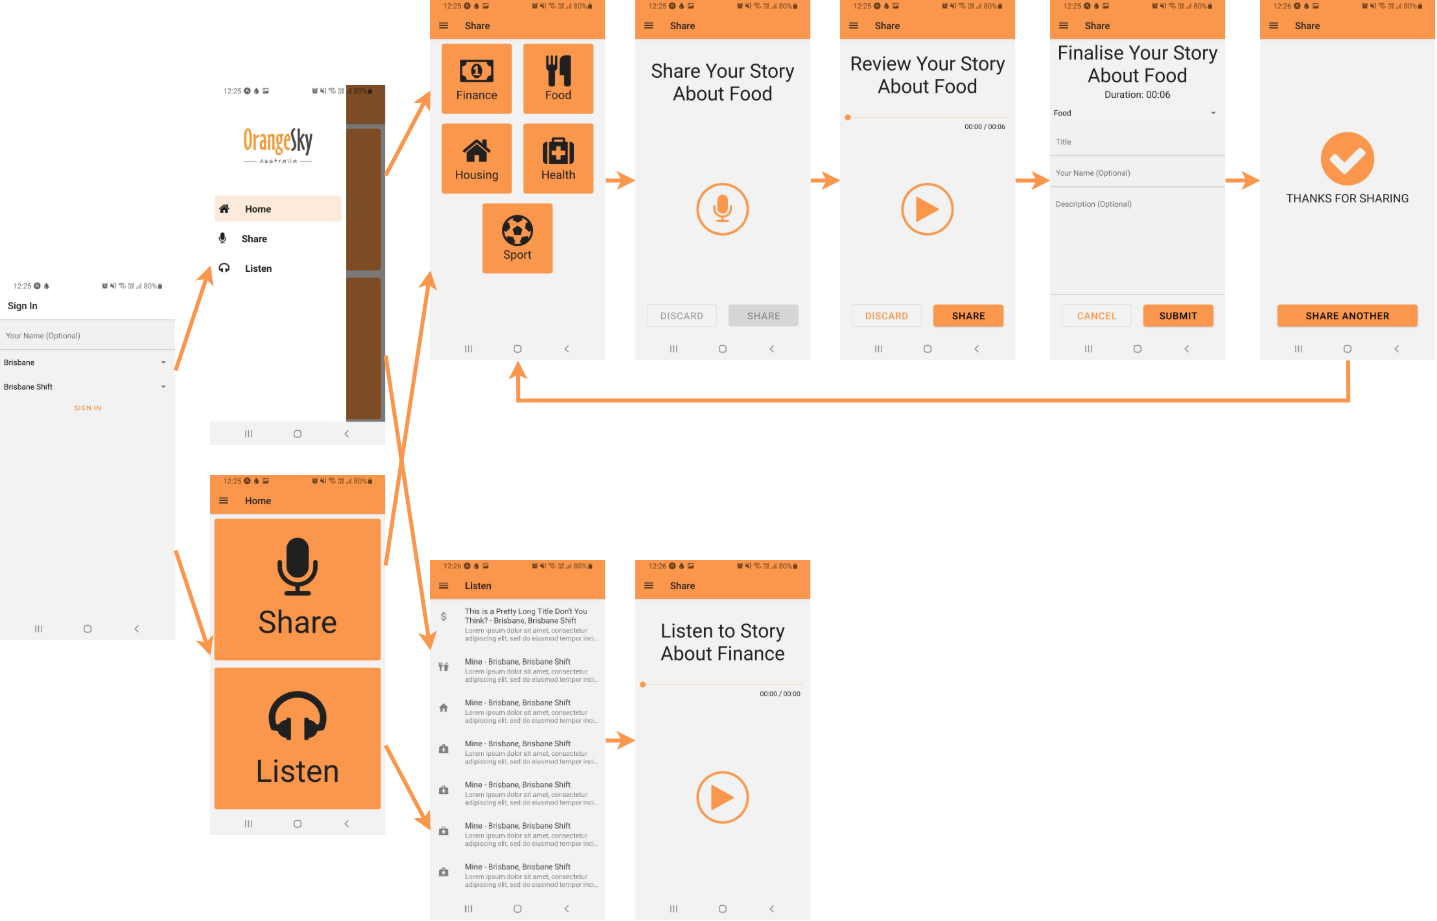
\includegraphics[width=\textwidth]{assets/designs/20200831-mockups.png}
    \caption{Final Prototype: Login \& Navigation (left), Share (top), Listen (bottom)}
    \label{finalprototype}
\end{figure}

Most notably different from our initial designs, beyond the visuals of the application, is the medium that is being utilised for story. Whilst our initial designs outlined a desire to capture stories through text, it was decided that this was potentially not conducive to the type of connection that we were hoping to establish in Orange Sky's service model. By shifting to voice recording as our collection medium, it was postulated that this would lead to the establishment of stronger empathy when listening to another individual's story. We also reason that collecting through voice recording is more in line with the expectations of an Orange Sky service, a service which is renowned and celebrated for its emphasis on conversations with those experiencing homelessness. Our results will look to discuss the accuracy of our assumptions around voice recording as the ideal medium, and recommendations may be made for future development in this space.

Most major differences in visuals can be simply put down to limitations in technical libraries, frameworks, and even ability. The only notable visual change that was intentionally made from the initial designs, was to incorporate less white, and more of Orange Sky's recognisable colour scheme. This was done to ensure that the application was in alignment with established branding, as well as to ensure that the application would be easily usable in harsh lighting conditions out in the field.

Other noteworthy changes from initial design include the simple \emph(Home) screen, implemented as two large buttons consuming the entire screen such that it is immediately clear to all users what the key functionalities of the application are. The templates and tips in story sharing have also been streamlined into a category system, allowing users to share and read stories within their own categories of interest. We propose that these categories are adjusted and expanded over time, as their use patterns becomes more apparent. Our voice recording interface is also designed to be as simple and intuitive as possible, utilising icons and design patterns that are commonplace in most audio based applications.

In landing at this final design, all that was now required was for the application to be made functional, before it could be finally sent out into the field with Orange Sky. Further details on these designs can also be found in Appendix \ref{appendix:design}.

\subsection{Technical Information}

In determining the appropriate technology stack to develop the application, the following factors were deemed critical:

\begin{itemize}
    \item \emph{Developer familiarity}: due to the desire for rapid prototyping
    \item \emph{Orange Sky familiarity and fit}: such that the application can be transferred into the organisation if desired
    \item \emph{Secure}: to ensure the safety of those experiencing homelessness, as well as to mitigate any organisational risks for Orange Sky
    \item \emph{Performant}: as it is important that the application can run on the older tablets utilised by Orange Sky without rapidly draining their batteries
    \item \emph{Portable}: ensuring the ease of deployment and the mitigation of any infrastructural difficulties in delivering the application
\end{itemize}

In consideration of the above requirements it was decided that the application would utilise \emph{PHP} on the back-end, supported by a \emph{MySQL} relational database. This would be accompanied by a \emph{React Native} application on the tablets, built using the \emph{Expo} tooling package.

\emph{PHP 7.4} is the standard back-end programming language within Orange Sky, and is also of most familiarity to us. Through diligent programming practices in alignment with industry standards, it is known that \emph{PHP} is satisfactory for providing the security, performance, and portability that is required. \emph{PHPStan} was utilised as an accompanying development tool to ensure the type safety and best practices were sufficient in our back-end code. This code was containerised and deployed in a cloud environment utilising \emph{Docker}, another tool in standard use within Orange Sky.

Alongside the containerised and deployed back-end code was positioned a \emph{MySQL} instance, locked down and only accessible by the networked back-end containers. A \emph{MySQL} for, \emph{MariaDB}, is in standard use at Orange Sky, and this is of little concern if our application is to be adopted.

The Android application itself was built using the open source \emph{Expo} platform which runs over the top of the standard \emph{React Native} development workflows. \emph{React Native} is in use at Orange Sky for the existing tablet applications. \emph{TypeScript} was also implemented in this application in an effort to provide compile time checks and linting, as well as bundling and optimisations benefits. An APK was built for distributing and installing the application.

\section{Delivery Strategy}

Given the scale of Orange Sky's services throughout Australia and New Zealand, it was determined that a number of different delivery strategies would be explored. With the differences in these strategies to be discussed and conclusions drawn as to their comparative effectiveness.

In general, all of these strategies revolve around the core concept of the application being installed on a tablet that is present on a regular Orange Sky shift. This application would then be introduced to those experiencing homelessness who were present on these shifts, in the hope that these individuals would engage with the application either by sharing their own experiences, or by listening and responding to someone else's.

The different variations of this core strategy that were to be tested are listed below:

\begin{itemize}
    \item \emph{Accompanying formal interviews}: Formal academic interviews were also being performed on Orange Sky shift at this time, as a component of an accompanying study. Asking an individual if they wish to participate in the application was to occur alongside the established interview process.
    \item \emph{Informally through researchers}: The application was to be introduced informally through general conversation and mingling by an academic researcher.
    \item \emph{Informally through volunteers}: The application was to be introduced informally through general conversation and mingling by an existing Orange Sky volunteer.
\end{itemize}

As previously mentioned, each of these strategies are assumed to have differing levels of success, and this will be discussed later in this report. Compounding the variations in strategies being trialled, the application was also to be distributed geographically throughout Australia in an effort to attract as much participation as possible, as well as to investigate the affect of sharing stories with individuals with whom one will likely never cross paths.

\section{Accompanying Work}

Alongside this project, work was also being conducted by two other students also under the supervision of Dr Vyas. Jay Almaraz and Stephen Pozzi were also fortunate enough to conduct field research with Orange Sky, and at times were also assisting in data collection for this study. Almaraz's work was primarily focused on the experiences of those experiencing homelessness with relation to the existing Orange Sky services. And Pozzi's work intended to investigate the impacts and experiences of temporary homelessness, particular as a result of the COVID-19 pandemic.